\documentclass[tikz,border=8pt]{standalone}
\usepackage{braket}

\begin{document}
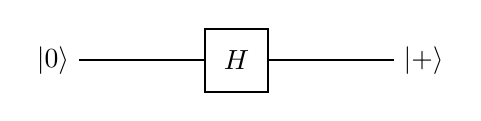
\begin{tikzpicture}[
  wire/.style={line width=0.8pt},
  gate/.style={draw,fill=white,line width=0.8pt,
    minimum width=0.8cm,minimum height=0.8cm,inner sep=0pt}
]
  \draw[wire] (0,0) -- (4,0);
  \node[left] at (0,0) {$\ket{0}$};
  \node[gate] at (2,0) {$H$};
  \node[right] at (4,0) {$\ket{+}$};
\end{tikzpicture}
\end{document}
